%% chapter8_slides.tex  -  Chapter 8: Bayesian Audit Outcome Model Selection Using Normalizing Flows
%% Bayesian Machine Learning in Quantitative Finance: Theory and Practical Applications
%% Mongwe, Mbuvha & Marwala (Springer, 2025)
%% Compile: pdflatex -interaction=nonstopmode chapter8_slides.tex  (twice)
\documentclass[aspectratio=169,10pt]{beamer}

\usetheme{Madrid}
\usecolortheme{seahorse}
\usefonttheme{professionalfonts}

%% packages
\usepackage{amsmath,amssymb,mathtools}
\usepackage{bm}
\usepackage{graphicx}
\usepackage{booktabs}
\usepackage{array}
\usepackage{listings}
\usepackage{xcolor}

\graphicspath{{figures/}}

%% listings style
\lstdefinestyle{pycode}{
  language=Python,
  basicstyle=\ttfamily\scriptsize,
  keywordstyle=\color{blue}\bfseries,
  commentstyle=\color{green!50!black}\itshape,
  stringstyle=\color{orange!80!black},
  numbers=left,
  numberstyle=\tiny\color{gray},
  numbersep=5pt,
  frame=single,
  backgroundcolor=\color{gray!7},
  tabsize=2,
  showstringspaces=false,
  breaklines=true,
  captionpos=b,
}
\lstset{style=pycode}

%% custom colours
\definecolor{myblue}{RGB}{33,102,172}
\definecolor{myorange}{RGB}{214,96,77}
\definecolor{mygreen}{RGB}{26,152,80}

%% footline, no navigation
\setbeamertemplate{footline}[frame number]
\setbeamertemplate{navigation symbols}{}
\setcounter{tocdepth}{1}

%%=============================================================================
\title[Bayesian ML in QF -- Ch.8]{Bayesian Machine Learning in Quantitative Finance}
\subtitle{Chapter 8: Audit Outcome Model Selection via Normalizing Flows}
\author{Based on Mongwe, Mbuvha \& Marwala}
\date{2025}

%%=============================================================================
\begin{document}

\begin{frame}
  \titlepage
\end{frame}

\begin{frame}{Chapter Outline}
  \tableofcontents
\end{frame}

%%=============================================================================
\section{8.1 Introduction}
%%=============================================================================

\begin{frame}[allowframebreaks]{8.1 The Audit Opinion Prediction Problem}

\textbf{Context.} Every year, the Auditor-General South Africa (AGSA) issues an \emph{audit opinion} on every municipality's financial statements. An opinion can be, roughly from best to worst:
\begin{itemize}
  \item \textbf{Unqualified} (``clean'') -- the financials are a fair representation, no material issues.
  \item \textbf{Unqualified with emphasis of matter} -- clean, but the auditor flags something to watch.
  \item \textbf{Qualified} -- specific, material problems were found.
  \item \textbf{Disclaimer} / \textbf{Adverse} -- the auditor could not form an opinion, or the financials are materially misstated.
\end{itemize}
AGSA reports repeatedly find that most South African municipalities still fail to obtain clean audits, raising real questions about financial management and internal controls.

\framebreak

\textbf{Why predict it?} If we could reliably predict a municipality's likely audit opinion \emph{before} the (costly, slow) audit is complete -- using only financial ratios that are cheap to compute -- then:
\begin{itemize}
  \item AGSA (or any auditor) could allocate scarce audit resources to the municipalities most likely to need deep scrutiny.
  \item Red flags could be raised early, using unaudited financials.
  \item The financial ratios that matter most (e.g.\ debt ratios, liquidity ratios) could be identified, informing policy.
\end{itemize}

This chapter is about a specific ingredient of that pipeline: given several candidate \emph{Bayesian} models for predicting audit opinions, \textbf{which model should we trust}? This is the model selection problem, and it is answered here using the \emph{Bayesian evidence}.

\end{frame}

\begin{frame}[allowframebreaks]{8.1 Machine Learning for Audit Outcomes: Prior Work}

Machine learning has already been used successfully to model audit opinions, both in South Africa and internationally:

\begin{itemize}
  \item \textbf{South Africa.} Marwala et al.\ (2023), Mongwe (2022) and Mongwe et al.\ (2021e) used a \emph{Bayesian} logistic regression trained with MCMC to predict municipal audit outcomes \emph{with uncertainty}, and to identify the most relevant financial ratios. Mabelane et al.\ (2023) compared logistic regression, random forests and SVMs, finding debt-to-operating-ratio, current ratio and net operating surplus margin to be consistently important.
  \item \textbf{International.} Studies in Greece (Spathis et al.; Kotsiantis et al.), the UK (Gaganis et al.), China (Deng \& Mei; Deng) and South Africa's listed-company space (Moepya et al.) have applied discriminant analysis, SVMs, ANNs, k-NN and unsupervised methods to detect qualified/fraudulent audit outcomes from financial ratios.
\end{itemize}

\framebreak

\textbf{The gap.} All of this work shows machine learning \emph{can} model audit opinions well. What it does not settle is: \emph{given several plausible models (e.g.\ different subsets of financial-ratio covariates), how do we reliably choose between them?}

This chapter addresses that model-selection question with a fully probabilistic framework: fit each candidate model with MCMC, then compare models using the \textbf{Bayesian evidence} -- a single number per model that automatically accounts for model complexity.

\end{frame}

\begin{frame}[allowframebreaks]{8.1 From Prediction to Principled Model Selection}

Bayesian inference gives us two things for a model $M$ with parameters $\theta$ and data $D$:
\begin{enumerate}
  \item the \textbf{posterior} $\mathbb{P}(\theta \mid D, M)$ -- what the data tell us about the parameters \emph{within} model $M$;
  \item the \textbf{evidence} (marginal likelihood) $\mathbb{P}(D \mid M)$ -- how well model $M$ as a whole explains the data, \emph{averaged over all parameter values}.
\end{enumerate}

Standard MCMC samplers (Metropolis--Hastings, MALA, HMC, NUTS) and variational inference are built to sample/approximate the posterior \emph{without ever needing the evidence} -- it is simply the normalizing constant they divide out. That is exactly the problem: for model comparison, this normalizing constant is precisely the quantity we need, and none of these methods hand it to us for free.

\framebreak

\textbf{Two families of fixes} exist in the literature:
\begin{itemize}
  \item \textbf{Nested sampling} (Skilling): the most widely used approach, but requires bespoke, low-dimensional-friendly sampling schemes and is often computationally expensive.
  \item \textbf{Harmonic mean estimators} (Newton \& Raftery, 1994): beautifully simple -- reuse the posterior samples you already have from \emph{any} MCMC run -- but historically plagued by an exploding-variance problem.
\end{itemize}

This chapter's contribution: use \textbf{normalizing flows} (which you met for density estimation in Chapter 5) to fix the harmonic mean estimator's instability -- the \emph{learnt harmonic mean estimator} of McEwen et al.\ (2021) and Polanska et al.\ (2023).

\end{frame}

\begin{frame}{8.1 Chapter Roadmap}
\begin{itemize}
  \item \textbf{8.2 Models} -- five nested Bayesian logistic regression models for audit opinions.
  \item \textbf{8.3 Bayesian Evidence Metric} -- what the evidence is and why it matters for model selection.
  \item \textbf{8.4 Harmonic Mean Estimator} -- the classical estimator, why it fails, and how normalizing flows (8.4.1) and MCMC samplers (8.4.2) fix/produce it.
  \item \textbf{8.5 Numerical Experiments} -- the South African municipal audit dataset and evaluation protocol.
  \item \textbf{8.6 Results and Discussion} -- does the evidence actually pick the model that generalizes best?
  \item \textbf{8.7 Conclusion.}
\end{itemize}
\vspace{0.3cm}
\textbf{Throughout these slides}, alongside the book's real results, we build our own small \emph{toy running example} -- two synthetic audit-outcome-style logistic regression models -- so every abstract formula gets a concrete number attached to it.
\end{frame}

%%=============================================================================
\section{8.2 Models}
%%=============================================================================

\begin{frame}[allowframebreaks]{8.2 Recap: Bayesian Logistic Regression}

\textbf{Intuition.} We want to predict a binary audit outcome $y_i \in \{0,1\}$ (e.g.\ 1 = unqualified/clean, 0 = not) from a vector of financial ratios $x_i$. Logistic regression models this with a linear score $\mathbf{w}^T x_i$ passed through a sigmoid link, and the Bayesian version treats the weight vector $\mathbf{w}$ as a random variable with a prior, rather than a single point estimate.

\begin{block}{Eq.\ (8.1): Negative Log-Likelihood Function}
\[
l(D \mid \mathbf{w}) = \sum_{i}^{N} y_i \log(\mathbf{w}^T x_i) + (1 - y_i)\log(1 - \mathbf{w}^T x_i)
\]
where $D = \{x, y\}$ is the data, $x$ are the covariates, $y$ is the binary target, $N$ is the number of observations, and $\mathbf{w}$ are the parameters to be estimated. (Here $\mathbf{w}^T x_i$ stands for the model's predicted probability, i.e.\ a sigmoid link is understood to have been applied to the linear predictor -- this is the standard Bernoulli log-likelihood for logistic regression.)
\end{block}

\framebreak

\textbf{Why this matters here.} Eq.\ (8.1) gives us the \emph{likelihood} $L(\theta_M) := \mathbb{P}(D \mid \theta, M)$ term that will appear everywhere in this chapter -- in the posterior, and (crucially) inside the evidence integral of Sect.\ 8.3 and the harmonic mean estimator of Sect.\ 8.4. Every one of the five candidate models in this chapter shares this same likelihood form; they differ only in \emph{which covariates} $x_i$ contains.

\end{frame}

\begin{frame}[allowframebreaks]{8.2 Prior and (Unnormalized) Posterior}

\begin{block}{Eq.\ (8.2): Un-normalized Posterior Log-Density}
\[
\ln \mathbb{P}(\mathbf{w} \mid D) = l(D \mid \mathbf{w}) + \ln \mathbb{P}(\mathbf{w} \mid \alpha)
\]
where $\ln \mathbb{P}(\mathbf{w}\mid\alpha)$ is the log of the prior placed on the parameters $\mathbf{w}$, given hyperparameters $\alpha$.
\end{block}

\textbf{Prior choice.} Following Mongwe et al.\ (2021e), each parameter $w_j$ is given an independent zero-mean Gaussian prior with standard deviation $\alpha = 10$:
\[
w_j \sim \mathcal{N}(0, \alpha^2), \qquad \alpha = 10.
\]
This is a weakly-informative prior: it expresses ``no strong opinion'' about the sign or magnitude of each coefficient, while still being proper (integrates to 1) -- which is essential, because an improper prior would make the evidence integral undefined.

\framebreak

\textbf{Why we stop at the un-normalized posterior.} Eq.\ (8.2) is exactly what an MCMC sampler needs (MALA/HMC/NUTS only ever require the \emph{gradient of the log of this un-normalized density}). It deliberately omits the normalizing constant $\mathbb{P}(D\mid M)$ -- the evidence -- because MCMC does not need it to produce posterior samples. The rest of this chapter is about recovering that missing constant \emph{after the fact}, from the very same MCMC samples.

\end{frame}

\begin{frame}[allowframebreaks]{8.2.1 Five Nested Candidate Models}

Using the same municipal-finance dataset as Mongwe et al.\ (2020b), the chapter compares five audit-opinion models built from different combinations of financial-ratio covariates:

\begin{table}
\centering\scriptsize
\begin{tabular}{cl}
\toprule
Model & Covariates \\
\midrule
1 & Debt to Community Wealth/Equity, Capital Expenditure \% Total Expenditure,\\
  & Debt to Total Operating Revenue, Current Ratio, Net Operating Surplus Margin \%\\
2 & Capital Expenditure \% Total Expenditure, Debt to Total Operating Revenue,\\
  & Current Ratio, Net Operating Surplus Margin \%\\
3 & Debt to Total Operating Revenue, Current Ratio, Net Operating Surplus Margin \%\\
4 & Debt to Total Operating Revenue, Current Ratio\\
5 & Debt to Total Operating Revenue\\
\bottomrule
\end{tabular}
\end{table}

\framebreak

\textbf{Nested structure.} Model 1 has the most parameters (5 covariates + intercept); each subsequent model drops exactly one covariate, down to Model 5 with a single covariate. Formally,
\[
\text{Model 5} \subset \text{Model 4} \subset \text{Model 3} \subset \text{Model 2} \subset \text{Model 1}.
\]
This nesting is deliberate: it lets us isolate the marginal value of adding \emph{one specific covariate at a time}.
\begin{itemize}
  \item Model $5 \to 4$: adds ``Current Ratio''.
  \item Model $4 \to 3$: adds ``Net Operating Surplus Margin \%''.
  \item Model $3 \to 2$: adds ``Capital Expenditure \% Total Expenditure''.
  \item Model $2 \to 1$: adds ``Debt to Community Wealth/Equity''.
\end{itemize}

\end{frame}

\begin{frame}[allowframebreaks]{8.2 Why Nested Models? Setting Up the Comparison}

\textbf{Intuition.} If we only looked at \emph{training-data fit} (e.g.\ likelihood or accuracy on the data used to fit the model), Model 1 would always look at least as good as Model 5, simply because it has strictly more flexibility -- more parameters can only help fit the training data, never hurt it. This is the classical over-fitting trap.

The \textbf{evidence} (Sect.\ 8.3) is designed to resist this trap: it does not just ask ``how well can this model's \emph{best} parameter setting fit the data?'' -- it asks ``\emph{averaged over all parameter values the prior finds plausible}, how well does this model explain the data?'' A model with many parameters has to spread its prior mass over a much larger space, so most of that mass corresponds to \emph{bad} fits -- diluting its average performance. This is how the evidence penalizes complexity automatically (Occam's razor), which is exactly why we need it to fairly compare Models 1--5.

\vspace{0.2cm}
\textbf{Toy running example (introduced now, used throughout).} In parallel with the book's five real audit-ratio models, we will build our own small \emph{toy} pair of logistic regression models on synthetic audit-like data: Model A (2 covariates) vs.\ Model B (4 covariates, with 2 extra covariates that carry no real signal) -- to see the same Occam's-razor logic play out with concrete numbers we compute ourselves.

\end{frame}

\begin{frame}[fragile]{8.2 Python: Bayesian Logistic Regression Log-Posterior}
\begin{lstlisting}
import numpy as np
from scipy.special import expit  # sigmoid

def log_likelihood(w, X, y):
    """Eq. (8.1)-style Bernoulli log-likelihood (numerically stable)."""
    logits = X @ w
    # y*log(sigmoid(logits)) + (1-y)*log(1-sigmoid(logits))
    return np.sum(y * logits - np.logaddexp(0.0, logits))

def log_prior(w, alpha=10.0):
    """Gaussian prior N(0, alpha^2) on each parameter -- Eq. (8.2)."""
    d = len(w)
    return (-0.5 * np.sum(w ** 2) / alpha ** 2
            - 0.5 * d * np.log(2 * np.pi * alpha ** 2))

def log_unnormalized_posterior(w, X, y, alpha=10.0):
    """Eq. (8.2): ln P(w|D) = l(D|w) + ln P(w|alpha), up to Z_M."""
    return log_likelihood(w, X, y) + log_prior(w, alpha)

# Model 1 uses X with 5 covariate columns (+ intercept),
# Model 5 uses X with just 1 covariate column (+ intercept) -- same
# log_unnormalized_posterior function, different design matrix X.
\end{lstlisting}
\end{frame}

%%=============================================================================
\section{8.3 Bayesian Evidence Metric}
%%=============================================================================

\begin{frame}[allowframebreaks]{8.3 Why Do We Need More Than the Posterior?}

You already know how to fit a Bayesian model's \emph{parameters}: sample from $\mathbb{P}(\theta \mid D, M)$ with MCMC. That answers ``given this model, what are plausible parameter values?''

It does \emph{not} answer a different, equally important question: ``\emph{is this the right model in the first place}, compared to some other model $M'$ with a different set of covariates, or a different functional form?''

\textbf{The key idea.} Instead of asking how well the \emph{best-fitting} parameter setting explains the data, Bayesian model comparison asks: \emph{averaged over every parameter value the prior considers plausible, how well does this entire model explain the data?} This single number is called the \textbf{evidence} or \textbf{marginal likelihood}. It lets us compare fundamentally different models (different covariates, even different families) on equal footing, and it automatically penalizes overly complex models -- Occam's razor built in, with no extra tuning knob required.

\end{frame}

\begin{frame}[allowframebreaks]{8.3 Bayes' Theorem for Model Parameters}

Estimating the posterior distribution $\mathbb{P}(\theta \mid D, M)$ of parameters $\theta$ for a given model $M$ and data $D$ is one of the core interests of Bayesian inference. Bayes' theorem expresses this:

\begin{block}{Eq.\ (8.3): Bayes' Theorem}
\[
\mathbb{P}(\theta \mid D, M) = \frac{\mathbb{P}(D \mid \theta, M)\, \mathbb{P}(\theta \mid M)}{\mathbb{P}(D \mid M)}
\]
where $\mathbb{P}(D\mid\theta,M)$ is the likelihood of the data, $\mathbb{P}(\theta\mid M)$ is the prior for the parameters, and $\mathbb{P}(D\mid M)$ is the evidence.
\end{block}

This is the same Bayes' rule you have used since Chapter 2/3 to build the posterior for a \emph{single} model. The new object of interest in this chapter is the denominator, $\mathbb{P}(D\mid M)$.

\end{frame}

\begin{frame}[allowframebreaks]{8.3 The Evidence: Averaging the Likelihood Over the Prior}

\begin{block}{Eq.\ (8.4): The Evidence (Marginal Likelihood)}
\[
\mathbb{P}(D \mid M) = \int_{\Omega_\theta} \mathbb{P}(D \mid \theta, M)\, \mathbb{P}(\theta \mid M)\, d\theta
\]
where $\theta$ may have a large dimension, and the integral is taken across the whole domain $\Omega_\theta$ of $\theta$.
\end{block}

\textbf{Reading the formula.} This is exactly Bayes' rule (8.3) rearranged -- since $\mathbb{P}(\theta\mid D,M)$ must integrate to 1 over $\theta$, integrating both sides of (8.3) against $d\theta$ isolates $\mathbb{P}(D\mid M)$ as the normalizing constant. It is literally the average likelihood, where the averaging weights are given by the prior.

\textbf{Occam's razor, automatically.} Even when two models can achieve the same \emph{best-case} likelihood, their evidence can differ substantially if their complexity differs: the prior distribution in the evidence integral inherently penalizes overly complicated models (Bishop, 1997; MacKay, 1992; Rasmussen \& Ghahramani, 2001).

\end{frame}

\begin{frame}[allowframebreaks]{8.3 Occam's Razor, Visualized}

\begin{center}
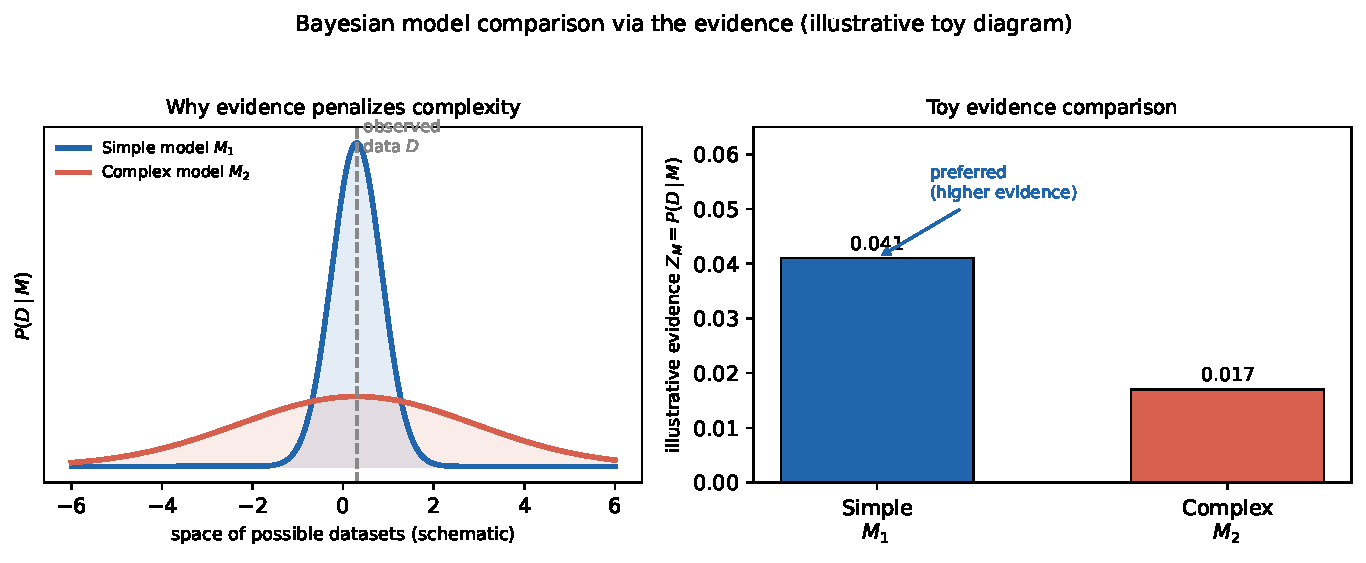
\includegraphics[width=0.92\linewidth]{fig1_occams_razor_evidence.pdf}
\end{center}

\textbf{Left panel (classic intuition).} Think of $\mathbb{P}(D\mid M)$ as a probability distribution \emph{over all datasets $M$ could have generated}. A simple model can only generate a narrow range of datasets, so it puts a tall, concentrated probability on those it \emph{can} explain. A complex model can generate a much wider range of datasets, so its probability mass is spread thin. If the observed data $D$ falls in the region both models can explain, the \emph{simpler} model wins because it was more ``confident'' about that outcome.

\textbf{Right panel.} A illustrative (made-up) toy evidence comparison consistent with the left panel: $Z_{M_1} = 0.041 > Z_{M_2} = 0.017$, so the simple model $M_1$ is preferred, even though both could fit the observed data reasonably well.

\end{frame}

\begin{frame}[allowframebreaks]{8.3 Shorthand Notation for the Rest of the Chapter}

For ease of reference, the following shorthand (Speagle, 2020) is used throughout the remainder of this chapter:

\begin{block}{Eq.\ (8.5): Shorthand Notation}
\[
\mathbb{P}(\theta_M) = \frac{L(\theta_M)\, \pi(\theta_M)}{Z_M}
\]
where $\mathbb{P}(\theta_M) := \mathbb{P}(\theta \mid D, M)$ is the posterior, $L(\theta_M) := \mathbb{P}(D \mid \theta, M)$ is the likelihood, $\pi(\theta_M) := \mathbb{P}(\theta \mid M)$ is the prior, and $Z_M := \mathbb{P}(D \mid M)$ is the evidence.
\end{block}

From the posterior $\mathbb{P}(\theta_M)$ one gets parameter estimates for a given model $M$ (this is what MCMC gives you directly); $Z_M$ is what lets you compare across models. This notation ($L$, $\pi$, $Z_M$) will be used in every formula from here on -- in particular the harmonic mean estimator of Sect.\ 8.4 targets $Z_M$ directly.

\end{frame}

\begin{frame}[allowframebreaks]{8.3 Comparing Models: The Bayes Factor}

\begin{block}{Eq.\ (8.6): Bayes Factor}
\[
B_{ij} := \frac{Z_{M_i}}{Z_{M_j}} \cdot \frac{\pi(M_i)}{\pi(M_j)}
\]
where $\pi(M_i)$ is the prior belief for model $i$.
\end{block}

If we have no reason to prefer one model over another \emph{a priori} (the usual case), $\pi(M_i) = \pi(M_j)$, so comparing models reduces to comparing their evidences directly: $B_{ij} = Z_{M_i}/Z_{M_j}$. Values of $B_{ij} > 1$ favor model $i$; note that $B_{ij} = 1/B_{ji}$.

\begin{block}{Table 8.1: Jeffreys' Scale for Interpreting $B_{ij}$}
\centering\scriptsize
\begin{tabular}{lll}
\toprule
$B_{ij}$ & $\ln B_{ij}$ & Strength of evidence\\
\midrule
$1 \le B_{ij} < 3$ & $0 \le \ln B_{ij} < 1.1$ & Weak\\
$3 \le B_{ij} < 20$ & $1.1 \le \ln B_{ij} < 3$ & Definite\\
$20 \le B_{ij} < 150$ & $3 \le \ln B_{ij} < 5$ & Strong\\
$150 \le B_{ij}$ & $5 \le \ln B_{ij}$ & Very strong\\
\bottomrule
\end{tabular}
\end{block}
(Nesseris \& Garcia-Bellido, 2013, as used throughout this chapter's results.)

\end{frame}

\begin{frame}[allowframebreaks]{8.3 Toy Running Example: Two Competing Audit Models}

To make everything concrete, alongside the book's real Models 1--5, we build a small synthetic ``audit-outcome-like'' dataset ($n=220$ toy municipalities, 4 standardized covariates) and two toy logistic regression models:

\begin{itemize}
  \item \textbf{Model A} (simple): covariates = \{debt-to-revenue, current-ratio-like\}, so $d=3$ parameters (with intercept).
  \item \textbf{Model B} (complex): covariates = \{debt-to-revenue, current-ratio-like, capex\%-like, net-op-margin-like\}, $d=5$ parameters. \emph{By construction}, the two extra covariates in Model B carry \textbf{no real signal} -- the synthetic labels only depend on the first two covariates.
\end{itemize}

This mirrors the book's actual Model 1 vs.\ Model 2 comparison in spirit (adding a covariate that turns out not to matter much), but with our own synthetic data and our own (simplified) evidence computation, so we can see the whole pipeline end to end. We will compute $Z_A$ and $Z_B$ once we have a concrete evidence-estimation tool in Sect.\ 8.4, and revisit the result in Sect.\ 8.6.

\end{frame}

\begin{frame}[fragile]{8.3 Python: Evidence via Grid Quadrature (Toy, Low-D)}
\begin{lstlisting}
import numpy as np
from scipy.special import expit

# For a LOW-dimensional toy model (e.g. 1-2 parameters), Eq. (8.4)
# can be approximated directly by brute-force numerical quadrature --
# useful as a ground truth to check estimators against (Sect. 8.4).

def log_unnorm_posterior_grid(B, W, x, y, alpha=10.0):
    """Evaluate ln[L(w)*pi(w)] on a grid of (intercept b, slope w)."""
    logits = B[..., None] + W[..., None] * x[None, None, :]
    loglik = np.sum(y[None, None, :] * logits
                     - np.logaddexp(0.0, logits), axis=-1)
    logprior = (-0.5 * (B ** 2 + W ** 2) / alpha ** 2
                - np.log(2 * np.pi * alpha ** 2))
    return loglik + logprior

def evidence_by_quadrature(b_grid, w_grid, x, y, alpha=10.0):
    BB, WW = np.meshgrid(b_grid, w_grid, indexing='ij')
    log_g = log_unnorm_posterior_grid(BB, WW, x, y, alpha)
    m = log_g.max()
    db, dw = b_grid[1]-b_grid[0], w_grid[1]-w_grid[0]
    Z = np.exp(m) * np.sum(np.exp(log_g - m)) * db * dw   # Eq. (8.4)
    return Z  # only feasible because the toy model has 2 parameters!
\end{lstlisting}
\end{frame}

%%=============================================================================
\section{8.4 Harmonic Mean Bayesian Evidence Estimator}
%%=============================================================================

\begin{frame}[allowframebreaks]{8.4 The Challenge: Evidence Is a Hard Integral}

Computing $Z_M = \int_{\Omega_\theta} L(\theta_M)\, \pi(\theta_M)\, d\theta$ (Eq.\ 8.4) directly is generally intractable: $\theta$ is often high-dimensional, and the integrand can vary wildly across $\Omega_\theta$. Plain MCMC integration might, in principle, be used, but even in very low dimensions this is unreliable in practice.

\textbf{Existing approaches:}
\begin{itemize}
  \item \textbf{Nested sampling} (static, diffusive, dynamic; Skilling, 2004/2006) -- the most widely used family, but needs custom samplers and is usually limited to low-dimensional problems.
  \item \textbf{Importance-sampling-based methods}, notably the \textbf{harmonic mean estimator} (Newton \& Raftery, 1994) -- the focus of this section.
\end{itemize}

\framebreak

\textbf{Why the harmonic mean estimator is appealing.} Unlike nested sampling, it needs \emph{only} samples from the posterior $\mathbb{P}(\theta_M)$ -- samples you likely \emph{already have} from whatever MCMC sampler (MALA, HMC, NUTS, \dots) or variational scheme you used to fit the model in the first place. There is no bespoke sampling scheme to design: it is a simple post-processing step on stored MCMC chains. This flexibility is also why it (or its ``learnt'' successor) can be extended to simulation-based inference, where an explicit likelihood may not even be available.

The catch -- covered next -- is that the classical version of this estimator can fail catastrophically.

\end{frame}

\begin{frame}[allowframebreaks]{8.4 The Idea Behind the Harmonic Mean Estimator}

\textbf{Intuition first.} We already have posterior samples $\theta^{(1)}, \dots, \theta^{(N)} \sim \mathbb{P}(\theta_M)$ from MCMC. Could some simple average of a quantity we can compute at each sample -- the likelihood $L(\theta^{(i)}_M)$ -- give us $Z_M$ directly, with no extra sampling? Newton and Raftery (1994) showed the answer is yes, provided you average the \emph{reciprocal} of the likelihood, not the likelihood itself.

We will now derive \emph{why} this works, from Bayes' rule alone -- and then see, with a tiny hand-worked example, exactly why this estimator is dangerous in practice.

\end{frame}

\begin{frame}[allowframebreaks]{8.4 Deriving the Harmonic Mean Identity, Step by Step}

\textbf{Step 1.} Start from Bayes' rule in the shorthand of Eq.\ (8.5):
\[
\mathbb{P}(\theta_M) = \frac{L(\theta_M)\,\pi(\theta_M)}{Z_M}.
\]

\textbf{Step 2.} Consider the posterior expectation of $1/L(\theta_M)$:
\[
\mathbb{E}_{\mathbb{P}(\theta_M)}\!\left[\frac{1}{L(\theta_M)}\right]
= \int \frac{1}{L(\theta_M)}\, \mathbb{P}(\theta_M)\, d\theta
= \int \frac{1}{L(\theta_M)} \cdot \frac{L(\theta_M)\,\pi(\theta_M)}{Z_M}\, d\theta.
\]

\textbf{Step 3.} The $L(\theta_M)$ terms cancel exactly:
\[
= \frac{1}{Z_M} \int \pi(\theta_M)\, d\theta = \frac{1}{Z_M} \cdot 1 = \frac{1}{Z_M},
\]
since the prior $\pi(\theta_M)$ is a proper probability density and integrates to 1.

\framebreak

\textbf{The harmonic mean identity.}
\[
\boxed{\ \mathbb{E}_{\mathbb{P}(\theta_M)}\!\left[\frac{1}{L(\theta_M)}\right] = \frac{1}{Z_M}\ }
\]

This is remarkable: an expectation \emph{taken entirely under the posterior} recovers the reciprocal evidence, with no extra integral to evaluate and no reference to the prior's normalization beyond ``it integrates to 1''. Approximate the left-hand side by a Monte Carlo average over posterior samples, and you have an estimator of $Z_M$. That is exactly what Eq.\ (8.7) does next.

\end{frame}

\begin{frame}[allowframebreaks]{8.4 The Harmonic Mean Estimator}

Writing $\rho_M := 1/Z_M$, Newton and Raftery's estimator replaces the exact expectation with a sample average over $N$ posterior draws $\theta_M^i \sim \mathbb{P}(\theta_M)$:

\begin{block}{Eq.\ (8.7): Harmonic Mean Evidence Estimator}
\[
\hat{\rho}_M = \frac{1}{N} \sum_{i=0}^{N} \frac{1}{L(\theta_M^i)}, \qquad \hat{Z}_M = \frac{1}{\hat\rho_M}
\]
where $N$ specifies the number of posterior samples $\theta_M^i$.
\end{block}

This is why it is called the \emph{harmonic} mean: $\hat Z_M$ is the harmonic mean of the sampled likelihood values $L(\theta_M^i)$ (the harmonic mean of a set of numbers is the reciprocal of the mean of their reciprocals). Simple to implement -- but, as Newton and Raftery themselves quickly discovered, the estimator's variance can be catastrophic. Let's see why with numbers.

\end{frame}

\begin{frame}[allowframebreaks]{8.4 Toy Numeric Example: 4 Posterior Samples by Hand}

Suppose (purely for illustration) we have drawn $N=4$ posterior samples, with made-up likelihood values:
\[
L(\theta^{(1)}) = 0.20,\quad L(\theta^{(2)}) = 0.15,\quad L(\theta^{(3)}) = 0.18,\quad L(\theta^{(4)}) = 0.01.
\]

\textbf{By hand:}
\[
\frac{1}{L(\theta^{(1)})}=5.0,\ \ \frac{1}{L(\theta^{(2)})}=6.67,\ \ \frac{1}{L(\theta^{(3)})}=5.56,\ \ \frac{1}{L(\theta^{(4)})}=100.0
\]
\[
\hat\rho_M = \frac{5.0+6.67+5.56+100.0}{4} = 29.31 \quad\Longrightarrow\quad \hat Z_M = \frac{1}{29.31} = 0.034
\]

\framebreak

\begin{center}
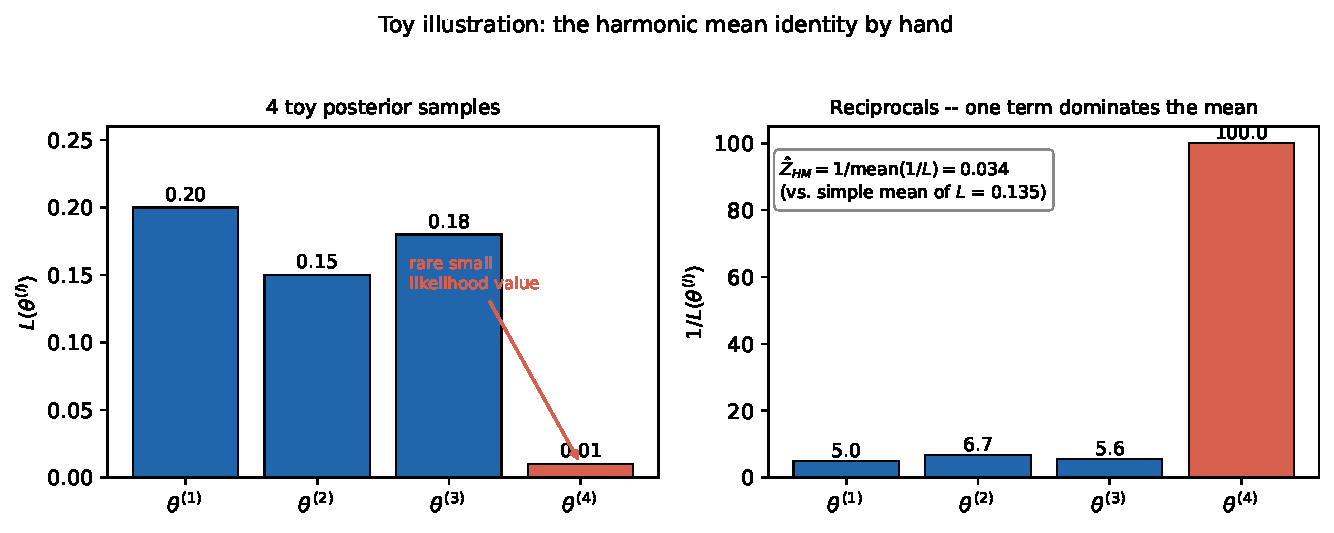
\includegraphics[width=0.92\linewidth]{fig2_toy4_harmonic_mean.pdf}
\end{center}

\textbf{The lesson.} The one atypically \emph{small} likelihood value, $L(\theta^{(4)})=0.01$, contributes $1/0.01=100$ to the sum -- roughly \textbf{20 times} the contribution of any other sample -- and single-handedly dominates the average. The resulting estimate $\hat Z_M = 0.034$ is far below the simple mean of the likelihoods ($\bar L = 0.135$), simply because \emph{one} sample happened to land somewhere the model fit poorly. A posterior sampler that occasionally wanders into the tails (which \emph{all} samplers do) will occasionally produce exactly this kind of outlier -- and every one of them destabilizes $\hat Z_M$.

\end{frame}

\begin{frame}[allowframebreaks]{8.4 Why It (Usually) Fails: An Importance-Sampling View}

Another way to understand the harmonic mean estimator is as \textbf{importance sampling}, where the sampling density is the posterior and the importance-sampling \emph{target} distribution is the prior:
\[
\mathbb{E}_{\pi(\theta_M)}[\, \cdot \, ] \approx \frac{1}{N}\sum_i \frac{\pi(\theta^{(i)})}{\mathbb{P}(\theta^{(i)}_M)} \cdot [\, \cdot \, ], \qquad \theta^{(i)} \sim \mathbb{P}(\theta_M).
\]

\textbf{The general rule for importance sampling to work well:} the \emph{sampling} density must have \emph{heavier tails} than the \emph{target} density -- otherwise the importance weights $\pi(\theta)/\mathbb{P}(\theta_M)$ can blow up in the sampling density's tails.

\textbf{The problem here.} New data always \emph{updates} (sharpens) our knowledge relative to the prior, so the posterior is typically \emph{narrower}-tailed than the prior, not broader. That means the sampling density (posterior) here has \emph{thinner} tails than the target (prior) -- exactly backwards from what importance sampling needs. Any posterior sample that lands in the posterior's own tail can carry a huge, destabilizing weight -- in the worst case, the estimator's variance is provably \textbf{infinite}.

\end{frame}

\begin{frame}[allowframebreaks]{8.4 Toy Simulation: How Bad Is the Instability?}

To see this concretely (not just abstractly), we build a toy 2-parameter Bayesian logistic regression (intercept $b$, slope $w$, Gaussian prior with $\alpha=10$, matching the book's prior), compute its \emph{true} evidence by brute-force grid quadrature (feasible here because $d=2$), and then repeat the naive harmonic mean estimator (Eq.\ 8.7) over 300 independent replicate draws of $N=60$ posterior samples each:

\begin{center}
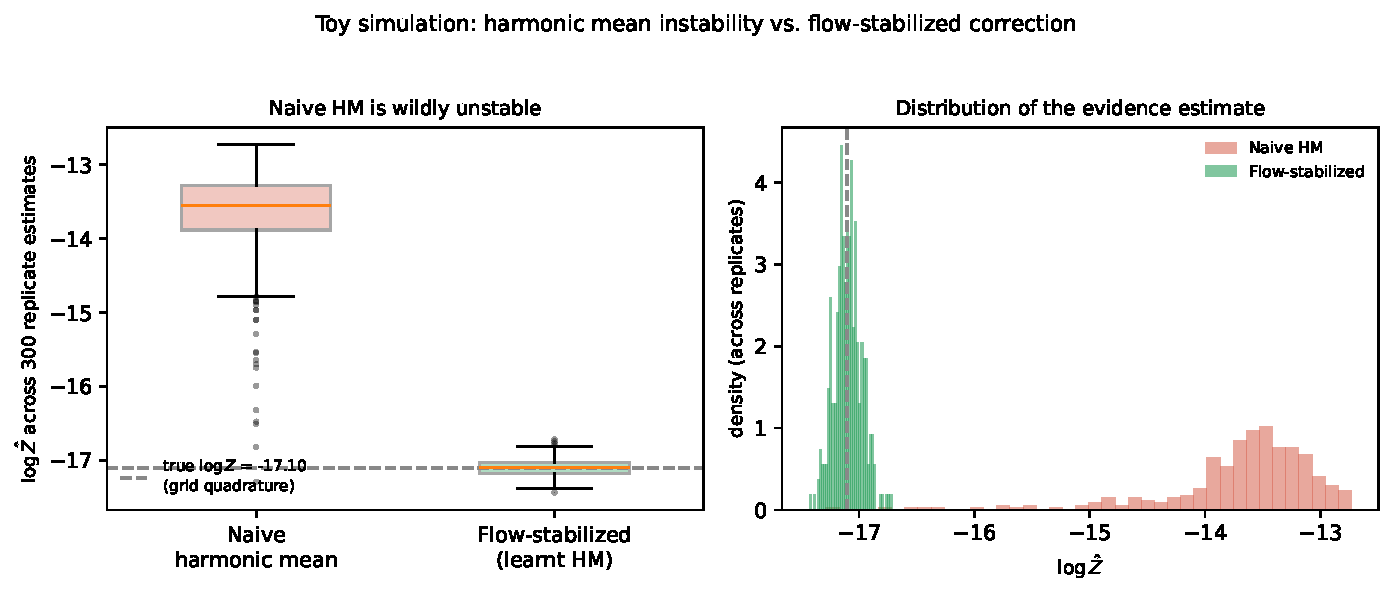
\includegraphics[width=0.92\linewidth]{fig3_harmonic_mean_variance.pdf}
\end{center}

\framebreak

\textbf{Our toy numbers.} Ground truth from grid quadrature: $\log Z_{\text{true}} = -17.10$.
\begin{itemize}
  \item \textbf{Naive harmonic mean}: mean $\log\hat Z = -13.69$, std.\ dev.\ $= 0.68$, range $[-17.29, -12.73]$ across replicates. It is not just noisy -- it is \textbf{severely biased upward}, overestimating the evidence by a factor of roughly $e^{3.4} \approx 30\times$ on average, precisely because occasional low-likelihood samples are down-weighting the estimate less than they should on some draws and more on others (a well-documented failure mode of this estimator).
  \item \textbf{Flow-stabilized (``learnt'') harmonic mean} (Sect.\ 8.4.1 mechanism, simplified here): mean $\log \hat Z = -17.10$, std.\ dev.\ $= 0.12$ -- centered right on the truth, with roughly \textbf{6$\times$ smaller spread}.
\end{itemize}
This toy simulation is our own illustrative construction -- but it reproduces exactly the qualitative failure the book describes for the classical estimator, and exactly the qualitative fix normalizing flows provide.

\end{frame}

%%=============================================================================
\subsection{8.4.1 Normalizing Flows}
%%=============================================================================

\begin{frame}[allowframebreaks]{8.4.1 Recap: Normalizing Flows}

\textbf{The fix in one sentence.} McEwen et al.\ (2021) showed that the instability above comes down to a bad choice of importance/target density; if instead we \emph{learn} a density whose probability mass is guaranteed to sit safely \emph{inside} the posterior (rather than relying on the prior, which is too broad), the same harmonic-mean-style estimator becomes stable. \textbf{Normalizing flows} (Chapter 5) are the tool used to learn that density.

\begin{block}{Eq.\ (8.8): Change of Variables}
\[
p(\theta) = q(z)\,\big|\det(J_T(z))\big|^{-1}
\]
where a vector $\theta$ of an unknown distribution $p(\theta)$ is expressed via a transformation $T$ of a vector $z$ sampled from a base distribution $q(z)$, i.e.\ $\theta = T(z)$ with $z \sim q(z)$, and $J_T(z)$ is the Jacobian of $T$.
\end{block}

\framebreak

\textbf{Why this works.} The base distribution $q(z)$ (often a simple Gaussian) is easy to sample from and has an easy-to-evaluate density. The whole transformation $T$ is built from a sequence of individually invertible, differentiable transformations, so the composed map is also invertible and differentiable -- letting us both sample from, and evaluate the density of, the resulting flexible distribution $p(\theta)$. Careful design keeps the Jacobian determinant cheap to compute.

\end{frame}

\begin{frame}[allowframebreaks]{8.4.1 Real NVP: Affine Coupling Layers}

This chapter uses the \textbf{real-valued non-volume-preserving (real NVP)} flow (Dinh et al., 2016), built from affine coupling layers. Split a $D$-dimensional input $z$ into $z_{1:d}$ and $z_{d+1:D}$ for some $d<D$:

\begin{block}{Eqs.\ (8.9)-(8.10): Affine Coupling Layer}
\[
y_{1:d} = z_{1:d}
\]
\[
y_{d+1:D} = z_{d+1:D} \odot \exp\big(s(z_{1:d})\big) + t(z_{1:d})
\]
where $\odot$ denotes elementwise (Hadamard) multiplication, and the scale $s$ and translation $t$ functions are typically neural networks with learnable parameters, taking $z_{1:d}$ as input.
\end{block}

\textbf{Key trick.} The first block passes straight through unchanged; the second block is only ever \emph{scaled and shifted} (never fed through a nonlinearity itself), so this transformation is trivially invertible, and its Jacobian is triangular -- its determinant is just the product of the diagonal (the exponentiated scale terms), making training tractable even for complex $s,t$ networks.

\end{frame}

\begin{frame}[allowframebreaks]{8.4.1 The Learnt Harmonic Mean Estimator}

\textbf{Putting it together.} Train a normalizing flow $q_\phi(\theta)$ on the posterior samples you already have, subject to a training objective (McEwen et al., 2021) that specifically \emph{guarantees the flow's probability mass stays inside the posterior's support} (rather than merely approximating the posterior everywhere, which can leak mass into thin-tailed regions and reintroduce the original instability). Then use $q_\phi$ in place of the prior inside the harmonic-mean-style importance identity.

\begin{center}
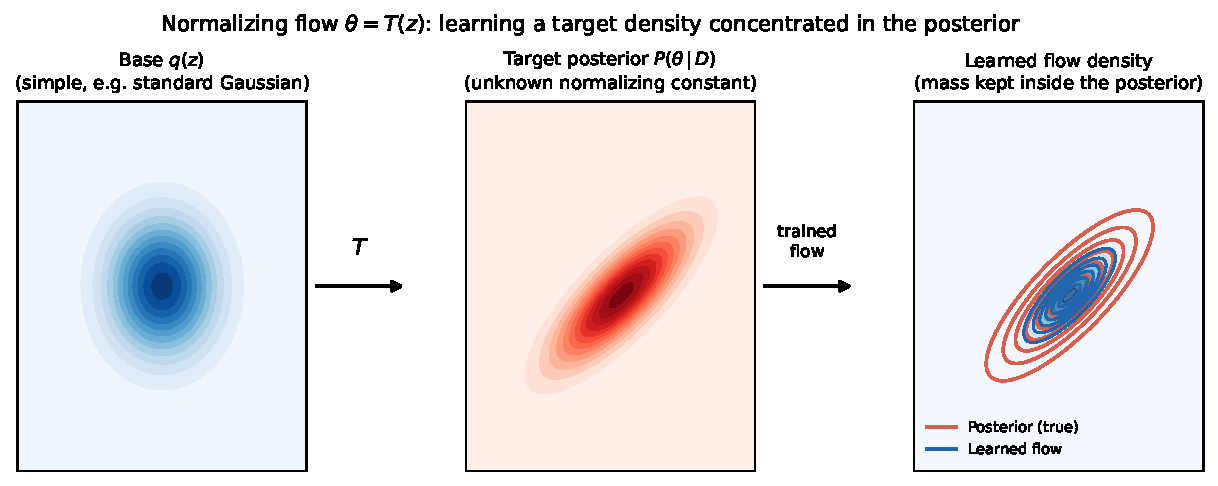
\includegraphics[width=0.85\linewidth]{fig4_normalizing_flow_schematic.pdf}
\end{center}

\framebreak

\textbf{Why concentrating the flow inside the posterior matters.} Recall the importance-sampling diagnosis from Sect.\ 8.4: instability arises when the importance/target density has \emph{fatter} tails than the posterior we are sampling from. A trained flow whose mass is deliberately \emph{narrower} than (and contained within) the posterior sidesteps this exactly -- there is no region where the target density is large but the posterior sampling density is small. This is the ``learnt harmonic mean estimator'' this chapter uses, and it scales to much higher dimensions than the bespoke schemes nested sampling requires.

\end{frame}

\begin{frame}[fragile]{8.4.1 Python: Real NVP Coupling Layer \& Flow-Corrected Evidence}
\begin{lstlisting}
import numpy as np

def affine_coupling_forward(z, d, s_net, t_net):
    """Eqs. (8.9)-(8.10): one real-NVP affine coupling layer."""
    z1, z2 = z[:d], z[d:]
    y1 = z1                                   # Eq. (8.9): passes through
    s, t = s_net(z1), t_net(z1)
    y2 = z2 * np.exp(s) + t                   # Eq. (8.10)
    log_det_jacobian = np.sum(s)              # triangular Jacobian!
    return np.concatenate([y1, y2]), log_det_jacobian

def flow_log_density(theta, z, log_det_jacobian_total, log_q_base):
    """Eq. (8.8): p(theta) = q(z) * |det J_T(z)|^{-1}  (in log-space)."""
    return log_q_base(z) - log_det_jacobian_total

def learnt_harmonic_mean_log_evidence(theta_samples, loglik_fn,
                                        logprior_fn, flow_log_density_fn):
    """Generalized harmonic mean using a flow g(theta) concentrated
    inside the posterior, in place of the (too-broad) prior."""
    log_ratios = np.array([
        flow_log_density_fn(th) - loglik_fn(th) - logprior_fn(th)
        for th in theta_samples
    ])
    from scipy.special import logsumexp
    log_rho_hat = logsumexp(log_ratios) - np.log(len(theta_samples))
    return -log_rho_hat   # log(Z_hat) = -log(rho_hat)
\end{lstlisting}
\end{frame}

%%=============================================================================
\subsection{8.4.2 Markov Chain Monte Carlo Algorithms}
%%=============================================================================

\begin{frame}[allowframebreaks]{8.4.2 Metropolis--Hastings and MALA}

The learnt harmonic mean estimator needs posterior samples -- \emph{any} valid MCMC chain will do. This chapter (as in earlier ones) uses MH, MALA, HMC and NUTS to produce them.

\textbf{Metropolis--Hastings (MH).} Uses a Gaussian proposal centered at the current state (a pure random walk). Simple, but produces strongly autocorrelated samples and hence slow convergence.

\begin{block}{Eq.\ (8.11): Langevin Dynamics (MALA)}
\[
d\mathbf{w}_t = \tfrac{1}{2} f'(\mathbf{w})\, dt + dZ_t
\]
where $\mathbf{w}$ are the parameters, $f'(\mathbf{w})$ is the first derivative of the target log-density $f(\mathbf{w})$ with respect to the parameters, and $Z_t$ is a Brownian motion process at fictitious time $t$.
\end{block}

\framebreak

The Metropolis-Adjusted Langevin Algorithm (MALA) uses first-order gradient information (the drift term above) to steer proposals \emph{towards} high-density regions, rather than wandering randomly like MH. Because the Langevin SDE (8.11) cannot generally be solved exactly, it is discretized (e.g.\ Euler--Maruyama), which introduces error -- corrected by an added Metropolis accept/reject step to preserve detailed balance and guarantee convergence to the correct posterior. MALA converges faster than MH, though its samples are still noticeably correlated.

\end{frame}

\begin{frame}[allowframebreaks]{8.4.2 Hamiltonian Monte Carlo}

HMC goes further: it introduces an auxiliary \emph{momentum} variable $\mathbf{p}$ (same dimension as $\mathbf{w}$) and simulates Hamiltonian dynamics, allowing much more distant, low-autocorrelation proposals.

\begin{block}{Eq.\ (8.12): Hamiltonian Dynamics}
\[
\frac{d\mathbf{w}}{dt} = \frac{\partial H(\mathbf{w},\mathbf{p})}{\partial \mathbf{p}}; \qquad
\frac{d\mathbf{p}}{dt} = -\frac{\partial H(\mathbf{w},\mathbf{p})}{\partial \mathbf{w}}
\]
where $H(\mathbf{w},\mathbf{p})$ is the Hamiltonian -- the total energy (potential energy from the target posterior, plus kinetic energy, typically a multivariate Gaussian in $\mathbf{p}$).
\end{block}

HMC has two steps: (1) integrate the dynamics (8.12) via the leapfrog scheme, and (2) a Metropolis correction for the resulting numerical (discretization) error.

\end{frame}

\begin{frame}[allowframebreaks]{8.4.2 Leapfrog Integration and the MH Correction}

\begin{block}{Eq.\ (8.13): Leapfrog Update}
\[
\mathbf{p}_{t+\epsilon/2} = \mathbf{p}_t + \frac{\epsilon}{2}\frac{\partial H(\mathbf{w}_t,\mathbf{p}_t)}{\partial \mathbf{w}}
\]
\[
\mathbf{w}_{t+\epsilon} = \mathbf{w}_t + \epsilon \mathbf{M}^{-1}\mathbf{p}_{t+\epsilon/2}
\]
\[
\mathbf{p}_{t+\epsilon} = \mathbf{p}_{t+\epsilon/2} + \frac{\epsilon}{2}\frac{\partial H(\mathbf{w}_{t+\epsilon},\mathbf{p}_{t+\epsilon/2})}{\partial \mathbf{w}}
\]
where $\epsilon$ is the discretization step size and $\mathbf{M}$ is the covariance matrix from the kinetic-energy term.
\end{block}

\begin{block}{Eq.\ (8.14): Metropolis Acceptance Probability}
\[
\mathbb{P}(\text{accept } \mathbf{w}^*) = \min\left(1, \frac{\exp(-H(\mathbf{w}^*,\mathbf{p}^*))}{\exp(-H(\mathbf{w},\mathbf{p}))}\right)
\]
\end{block}
HMC's tuning parameters -- step size $\epsilon$ and trajectory length -- are notoriously fiddly: too short a trajectory behaves like a random walk (MH-like), too long wastes computation tracing paths back on themselves.

\end{frame}

\begin{frame}[allowframebreaks]{8.4.2 NUTS and Dual Averaging}

The \textbf{No-U-Turn Sampler (NUTS)} removes the need to hand-tune trajectory length: it iteratively extends the trajectory until it starts to double back on itself (a ``U-turn'', $(\mathbf{w}^*-\mathbf{w})\times\mathbf{p}\le 0$) or the Hamiltonian diverges, then uses slice sampling to pick a point along the resulting path -- all without sacrificing detailed balance.

\begin{block}{Eqs.\ (8.15)-(8.16): Dual Averaging for the Step Size}
\[
\epsilon_{t+1} \leftarrow \mu - \frac{\sqrt{t}}{\gamma}\cdot\frac{1}{t+t_0}\sum_{i=1}^{t} H_i, \qquad
\bar\epsilon_{t+1} \leftarrow \eta_t \epsilon_{t+1} + (1-\eta_t)\bar\epsilon_t
\]
\[
\mathbb{E}[H_t] = \mathbb{E}[\delta - \alpha_t] = 0
\]
where $\eta_t$ is a decaying adaptation rate, $\gamma$ regulates convergence toward $\mu$, $H_t$ is the gap between the target acceptance rate $\delta$ and actual acceptance $\alpha_t$, and $\mu$ is a free parameter.
\end{block}
Typical settings: $\mu=\log(10\epsilon_0)$, $\bar\epsilon_0=1$, $\bar H_0=0$, $\gamma=0.05$, $t_0=10$, $\kappa=0.75$, $\epsilon_0=0.0001$ -- the same settings this chapter uses. NUTS is at least as efficient as a well-tuned HMC, without requiring the costly tuning runs HMC needs.

\end{frame}

\begin{frame}[fragile]{8.4.2 Python: MALA Step and HMC Leapfrog Integrator}
\begin{lstlisting}
import numpy as np

def mala_step(w, grad_log_post, step_size, rng):
    """One Metropolis-Adjusted Langevin Algorithm step -- Eq. (8.11)."""
    grad = grad_log_post(w)
    w_prop = w + 0.5 * step_size**2 * grad + step_size * rng.normal(size=w.shape)
    return w_prop  # (Metropolis accept/reject against detailed balance omitted)

def leapfrog(w, p, grad_log_post, step_size, n_steps, mass_inv=1.0):
    """HMC leapfrog integrator -- Eq. (8.13)."""
    p = p + 0.5 * step_size * grad_log_post(w)         # half-step momentum
    for _ in range(n_steps):
        w = w + step_size * mass_inv * p               # full-step position
        if _ != n_steps - 1:
            p = p + step_size * grad_log_post(w)        # full-step momentum
    p = p + 0.5 * step_size * grad_log_post(w)          # final half-step
    return w, p

def hmc_accept_prob(H_star, H_current):
    """Eq. (8.14): Metropolis correction for leapfrog's discretization error."""
    return min(1.0, np.exp(-H_star + H_current))
\end{lstlisting}
\end{frame}

%%=============================================================================
\section{8.5 Numerical Experiments}
%%=============================================================================

\begin{frame}[allowframebreaks]{8.5.1 The South African Municipal Audit Dataset}

Model selection is performed on a South African \textbf{municipal finance dataset} -- the same data used by Mongwe et al.\ (2020b) to study how well financial ratios identify financial-statement fraud.

\begin{itemize}
  \item \textbf{Source}: South African National Treasury (\texttt{municipaldata.treasury.gov.za}).
  \item \textbf{Coverage}: 2012--2018, $N = 1560$ observations of audited municipal financial statements and audit findings.
  \item \textbf{Split}: 70--30 train/test split, based on \emph{time} (not a random shuffle) -- so the test set genuinely represents ``the future'' relative to training.
  \item \textbf{Covariates}: 12 financial ratios described in Table 8.2 of the book (e.g.\ debt-to-community-wealth/equity, capital expenditure \% total expenditure, current ratio, net operating surplus margin \%, and others) -- Models 1--5 (Sect.\ 8.2) use different subsets of these.
\end{itemize}

\framebreak

\textbf{Target variable.} Raw audit opinions come in several categories (book's Fig.\ 8.1): qualified (28\%), unqualified\_emphasis\_of\_matter (41\%), unqualified (14\%), disclaimer (14\%), adverse (2\%), outstanding ($\approx$0\%). For modeling, this is collapsed into a \textbf{binary} target:
\[
y = \begin{cases} 1 & \text{unqualified opinion} \\ 0 & \text{not unqualified} \end{cases}
\]
Grouping ``unqualified'' with ``unqualified\_emphasis\_of\_matter'' gives $14\%+41\%=55\%$ of observations in the positive class -- a fairly \textbf{balanced} binary dataset.

\end{frame}

\begin{frame}[allowframebreaks]{8.5.2 Evaluation Protocol and MCMC/Flow Settings}

\textbf{Predictive metric.} Area Under the ROC Curve (AUC) on the held-out (time-based) test set, for every model and every MCMC sampler.

\textbf{MCMC settings} (identical across MALA, HMC, NUTS, for a fair comparison):
\begin{itemize}
  \item Pre-conditioning matrix $\mathbf{M} = \mathbf{I}$ (the typical default in practice).
  \item 10 independent chains, 6000 samples per chain, 1000-sample burn-in -- sufficient for convergence across all models (verified by trace plots).
  \item HMC: 25 leapfrog steps per proposal.
  \item Step sizes tuned via dual averaging (Eq.\ 8.15) to hit target acceptance rates: \textbf{60\%} for MALA, \textbf{80\%} for HMC and NUTS.
\end{itemize}

\framebreak

\textbf{Normalizing-flow settings for the learnt harmonic mean estimator:} a real NVP flow with \textbf{6 scaled coupling layers followed by 2 unscaled layers}, trained with a \textbf{temperature of 0.8} (a common trick to sharpen/concentrate the learned density -- consistent with the requirement in Sect.\ 8.4.1 that the flow's mass stay safely inside the posterior).

This identical protocol is applied to all five Models 1--5, so any differences in evidence or AUC in Sect.\ 8.6 reflect genuine differences between the models, not differences in how they were fit.

\end{frame}

%%=============================================================================
\section{8.6 Results and Discussion}
%%=============================================================================

\begin{frame}[allowframebreaks]{8.6 Log Evidence and Test AUC Across Models}

\begin{block}{Table 8.3: Log Evidence (Training Data) and AUC (Test Data)}
\centering\scriptsize
\begin{tabular}{lccccc}
\toprule
Metric & Model 1 & Model 2 & Model 3 & Model 4 & Model 5\\
\midrule
Log evidence (MALA) & $-909.86$ & $\mathbf{-908.91}$ & $-921.27$ & $-923.23$ & $-950.63$\\
Log evidence (HMC)  & $-910.15$ & $\mathbf{-908.996}$ & $-921.31$ & $-923.20$ & $-950.62$\\
Log evidence (NUTS) & $-910.16$ & $\mathbf{-908.995}$ & $-921.33$ & $-923.21$ & $-950.62$\\
Test AUC (MALA) & $0.7391$ & $\mathbf{0.7419}$ & $0.7386$ & $0.7358$ & $0.6734$\\
Test AUC (HMC)  & $\mathbf{0.7402}$ & $0.7401$ & $0.7385$ & $0.7358$ & $0.6734$\\
Test AUC (NUTS) & $\mathbf{0.7401}$ & $\mathbf{0.7401}$ & $0.7383$ & $0.7355$ & $0.6734$\\
\bottomrule
\end{tabular}
\end{block}
Bold = best (outperforming) entry per row. All log-evidence values are (as expected) large negative numbers -- the joint likelihood of $\sim$1092 training observations is astronomically small -- so \textbf{closer to zero (less negative) is better}.

\framebreak

\textbf{Headline result.} MALA, HMC and NUTS \textbf{agree closely} on the log evidence and AUC for every model -- the evidence estimate is not an artifact of which sampler produced the posterior samples. Across all three samplers:
\begin{itemize}
  \item \textbf{Model 2 has the highest (best) log evidence}, with \textbf{Model 1 a close second}.
  \item \textbf{Model 5 has the lowest (worst) log evidence} -- by a wide margin.
  \item The AUC ranking tracks the evidence ranking closely: Model 2 and Model 1 achieve the highest test AUC, Model 5 the lowest.
\end{itemize}
This is the central validation of the whole chapter: \textbf{a metric computed purely from training data (the evidence) successfully predicts which model will generalize best to unseen data.}

\end{frame}

\begin{frame}[allowframebreaks]{8.6 Occam's Razor in Action: Model 1 vs.\ Model 2}

Recall Model 1 has \emph{one more} covariate than Model 2 (``Debt to Community Wealth/Equity''), yet:
\begin{itemize}
  \item Model 1's log evidence ($-909.86$ for MALA) is \emph{lower} than Model 2's ($-908.91$) -- despite Model 1 being strictly more flexible.
  \item Their test AUCs are nearly identical ($0.7391$ vs.\ $0.7419$ for MALA).
\end{itemize}
This is Occam's razor at work \emph{exactly as promised in Sect.\ 8.3}: the evidence metric penalizes Model 1 for its extra parameter, because that parameter does not earn its keep in predictive performance -- even though nothing forced this outcome; the evidence naturally selected the simpler model once the extra covariate stopped adding value.

\vspace{0.2cm}
Symmetrically, \textbf{Model 5} (the single-covariate model) has by far the lowest evidence \emph{and} the lowest AUC ($0.6734$) -- so the evidence metric also correctly identifies genuinely under-specified, poor-performing models, not just penalizes complexity for its own sake.

\end{frame}

\begin{frame}[allowframebreaks]{8.6 Pairwise Bayes Factors (Table 8.4)}

\begin{block}{Table 8.4: Pairwise Log Bayes Factors (MALA Log Evidence)}
\centering\scriptsize
\begin{tabular}{lccccc}
\toprule
 & Model 1 & Model 2 & Model 3 & Model 4 & Model 5\\
\midrule
Model 1 & $\times$ & & & & \\
Model 2 & $-0.94$ & $\times$ & & & \\
Model 3 & $11.41$ & $12.36$ & $\times$ & & \\
Model 4 & $13.38$ & $14.32$ & $1.96$ & $\times$ & \\
Model 5 & $40.77$ & $41.72$ & $29.36$ & $27.40$ & $\times$\\
\bottomrule
\end{tabular}
\end{block}
Entry at (row, col) = log Bayes factor of the \emph{column} model vs.\ the \emph{row} model. E.g.\ row Model 4, column Model 2: $\ln B_{2,4} = 14.32$.

\textbf{Reading it via Jeffreys' scale (Table 8.1):}
\begin{itemize}
  \item Model 2 vs.\ Model 1: $|\ln B| = 0.94 < 1.1$ $\Rightarrow$ only \textbf{weak} evidence for Model 2 -- they are genuinely close.
  \item Model 2 vs.\ Models 3, 4, 5: $\ln B \in \{12.4, 14.3, 41.7\}$, all $\gg 5$ $\Rightarrow$ \textbf{very strong} evidence favoring Model 2.
\end{itemize}
Since Models 1--4 are all extensions of Model 5, this table also quantifies the value of each added covariate -- e.g.\ adding ``Current Ratio'' (Model $5\to4$) yields $\ln B \approx 27$--$29$: a very strong, clearly justified improvement.

\end{frame}

\begin{frame}[allowframebreaks]{8.6 Sampling Efficiency Across Models and Samplers}

Figures 8.2--8.4 in the book report effective sample size (ESS) and time-normalized ESS for MALA, HMC and NUTS, across all five models.

\begin{itemize}
  \item \textbf{MALA and HMC}: Model 5 (fewest parameters, $d=1$) has the \emph{highest} raw ESS, decreasing roughly monotonically as more covariates (and parameters) are added up to Model 1.
  \item \textbf{NUTS}: interestingly, this pattern \emph{reverses} -- Model 5 has the \emph{lowest} raw ESS with NUTS, while Model 1 has the highest.
  \item \textbf{Time-normalized ESS (ESS/execution time)}: all three samplers agree that Model 5 is by far the most efficient per unit of compute -- unsurprising, since fewer parameters means cheaper leapfrog/gradient computations per iteration.
\end{itemize}

The takeaway: \emph{raw} sampling efficiency does not tell you which model is scientifically better -- Model 5 samples fastest and most efficiently, yet Sect.\ 8.6's evidence and AUC results show it is by far the \emph{worst} model for actually predicting audit outcomes.

\end{frame}

\begin{frame}[allowframebreaks]{8.6 Convergence and ROC Diagnostics}

Figures 8.5--8.7 show, for each of MALA/HMC/NUTS: (a) ROC curves and AUC for all 5 models on the test set, and (b) negative log-likelihood trace plots over the MCMC run (a convergence diagnostic).

\begin{itemize}
  \item \textbf{Convergence}: negative log-likelihood trace plots are stable (flat, well-mixed) across all models and all three samplers, confirming the 1000-sample burn-in and 6000-sample chains were adequate.
  \item \textbf{ROC/AUC}: consistent with Table 8.3 -- Models 1 and 2 sit at the top (AUC $\approx 0.74$), Models 3 and 4 slightly behind, and Model 5's ROC curve is visibly closer to the diagonal ``no-skill'' line (AUC $\approx 0.67$).
  \item All three MCMC methods (MALA, HMC, NUTS) produce \textbf{near-identical} predictive performance for every model -- the choice of sampler does not materially change the conclusions, only the sampling efficiency (previous slide).
\end{itemize}

\end{frame}

\begin{frame}[allowframebreaks]{8.6 Corner Plots: Posterior vs.\ Concentrated Flow}

Figures 8.8--8.10 overlay, for every model and every MCMC method, the sampled posterior (red, solid) against the trained real-NVP flow's density (blue, dashed) in corner-plot form.

\textbf{Consistent finding across all 15 model$\times$sampler combinations:} the flow's probability mass is \textbf{visibly narrower and confined inside} the posterior's support -- exactly the property Sect.\ 8.4.1 argued is \emph{necessary} for the learnt harmonic mean estimator to have low variance (avoiding the importance-sampling tail mismatch that sank the naive estimator).

This is why Table 8.3's log-evidence values are trustworthy: the flow was not just fit for its own sake, its fit was verified (visually, via these corner plots) to satisfy the ``contained within the posterior'' condition needed for a reliable evidence estimate -- for every one of the five models, using every one of the three MCMC samplers.

\end{frame}

\begin{frame}[allowframebreaks]{8.6 Back to the Toy Running Example}

Returning to our toy Model A (2 covariates) vs.\ Model B (4 covariates, 2 of them pure noise) from Sect.\ 8.3, we estimate each model's evidence via a Laplace (Gaussian) approximation at the MAP -- a classical, simple alternative way to approximate the evidence, useful here to get concrete numbers quickly:

\begin{center}
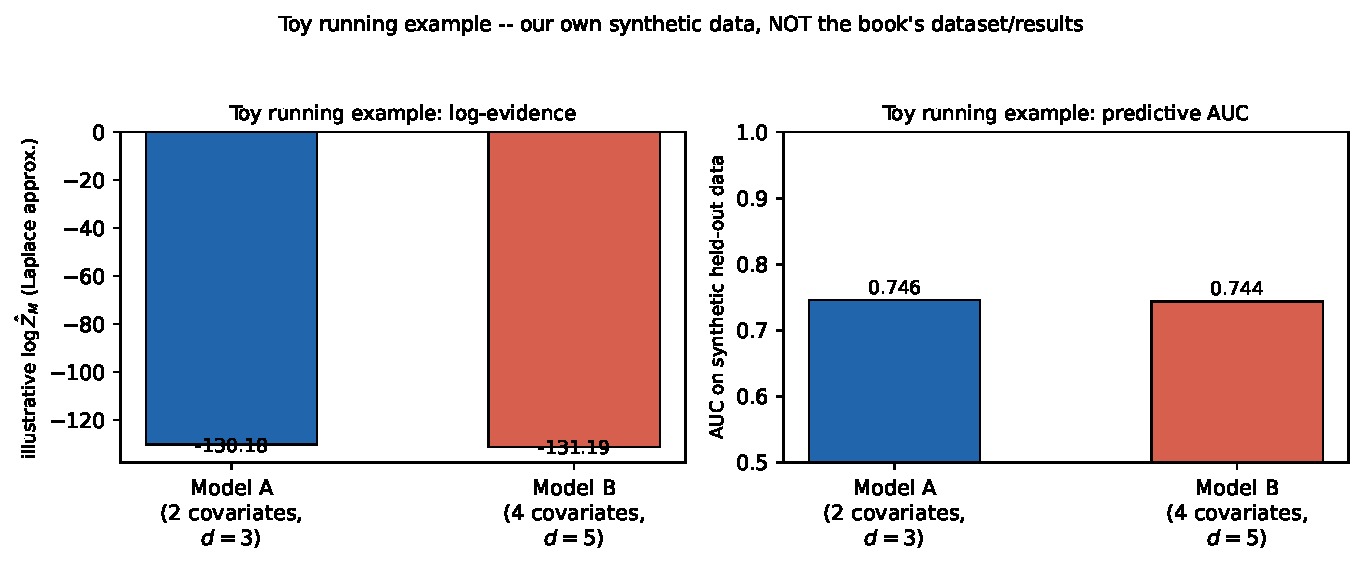
\includegraphics[width=0.9\linewidth]{fig5_toy_running_example.pdf}
\end{center}

\framebreak

\textbf{Our toy numbers:} $\log \hat Z_A = -130.18$ ($d=3$), $\log \hat Z_B = -131.19$ ($d=5$), giving $\ln B_{A,B} = \log\hat Z_A - \log\hat Z_B = 1.01$. By Jeffreys' scale (Table 8.1), $1.01 < 1.1$ is only \textbf{weak} evidence favoring the simpler Model A -- consistent with the held-out AUC (Model A: $0.746$ vs.\ Model B: $0.744$ -- nearly identical, Model A very slightly better).

\textbf{This mirrors the book's real Model 1 vs.\ Model 2 result almost exactly}: a genuinely uninformative extra covariate barely changes predictive performance, and the evidence metric reflects this with a small, ``weak'' Bayes factor rather than dramatically penalizing the larger model -- Occam's razor is a matter of degree, not an automatic veto on complexity. (As always: this is \emph{our own} toy simulation and Laplace approximation, not the book's dataset, models or harmonic-mean-based results.)

\end{frame}

%%=============================================================================
\section{8.7 Conclusion}
%%=============================================================================

\begin{frame}[allowframebreaks]{8.7 Conclusion}

This chapter tackled \textbf{Bayesian model selection for audit-opinion prediction} in South African municipalities:

\begin{itemize}
  \item Five nested Bayesian logistic regression models (Sect.\ 8.2), differing only in which financial-ratio covariates they include.
  \item Model comparison via the \textbf{Bayesian evidence} (Sect.\ 8.3) -- a single number per model that averages likelihood over the prior and automatically penalizes unnecessary complexity.
  \item The evidence estimated via the \textbf{learnt harmonic mean estimator}, using \textbf{normalizing flows} (real NVP) to fix the notorious instability of the classical harmonic mean estimator (Sect.\ 8.4), with posterior samples supplied by MALA, HMC and NUTS.
  \item \textbf{Results}: the evidence (computed purely from training data) successfully identified the model (Model 2) that also generalizes best on unseen data (AUC), and correctly penalized both an unnecessary extra covariate (Model 1) and a badly under-specified model (Model 5).
\end{itemize}

\framebreak

\textbf{Bigger picture.} This framework is not specific to logistic regression or to audit opinions -- it extends naturally to more complex models (e.g.\ deep neural networks) and more advanced samplers (e.g.\ Riemannian-manifold MCMC), wherever you need to compare fundamentally different Bayesian models on equal footing.

\vspace{0.3cm}
\textbf{Looking ahead.} Chapter 9 turns to a related but distinct problem in the same South African municipal setting: modeling \emph{unauthorized expenditure} using a Bayesian MCMC framework, again with the goal of identifying the most relevant variables -- this time from \emph{unaudited} financial statements.

\end{frame}

\end{document}
